\documentclass[a4paper,11pt,titlepage]{article}
\parskip 3pt

%% %%%%%%%%%%%%%%%%%%%% BEGIN PACKAGES %%%%%%%%%%%%%%%%%%%%

%%\usepackage[top=1in, bottom=1in, left=1in, right=1in]{geometry}

\usepackage{fullpage}
\usepackage{url}
\usepackage{hyperref}
\hypersetup{pdfborder=0 0 0}

%% Images
\usepackage{graphicx}

%% Side-by-side images
\usepackage{subfig}

%% Drawing trees and other stuff
\usepackage{tikz}
\usetikzlibrary{trees,arrows}
\usepackage{amssymb}

%% Pseudocode
\usepackage[noend]{algorithmic}
\algsetup{indent=1.5em}

%% Linux Libertine
\usepackage[T1]{fontenc}
\usepackage{libertine}
\renewcommand*\oldstylenums[1]{{\fontfamily{fxlj}\selectfont #1}}

%% %%%%%%%%%%%%%%%%%%%% END PACKAGES %%%%%%%%%%%%%%%%%%%%


%% %%%%%%%%%%%%%%%%%%%% BEGIN COMMANDS %%%%%%%%%%%%%%%%%%%%

\newcommand{\mailto}[1]{\href{mailto:#1}{\texttt{#1}}}

\let\stdsection\section         % because LaTeX cannot handle
                                % recursive commands
\renewcommand{\section}{\newpage\stdsection}

\let\tikzsquare\square
\renewcommand{\square}{\ensuremath\tikzsquare}

\newcommand{\FADE}{\texttt{FADE}\ }

\newcommand{\code}[1]{\texttt{#1}}

%% %%%%%%%%%%%%%%%%%%%% END COMMANDS %%%%%%%%%%%%%%%%%%%%

%% %%%%%%%%%%%%%%%%%%%% BEGIN COLORS %%%%%%%%%%%%%%%%%%%%

\definecolor{cffffff}{RGB}{255,255,255}
\definecolor{c787aff}{RGB}{120,122,255}
\definecolor{cff7374}{RGB}{255,115,116}
\definecolor{c79ff79}{RGB}{121,255,121}
\definecolor{cff7374}{RGB}{255,115,116}
\definecolor{c7372ff}{RGB}{115,114,255}

%% %%%%%%%%%%%%%%%%%%%% END COLORS %%%%%%%%%%%%%%%%%%%%


%% Final Report — due: 9th Jan 2012, at 11:00
%% Contents for Final Report: The project report should not be longer than 45 pages, and might be organized according to the following structure:

%% A. High Level, Nontechnical Description Why you should buy this product/listen to this presentation? What is the functionality of the product?
%% B. Short Technical Description
%% Short introduction into technologies used
%% Design of your software, possibly including a diagram of the major components of the project
%% Main achievements
%% C. Software Engineering Issues:
%% What technology was used and why; what other technology was considered but not used and why
%% Any technical challenges encountered and how addressed
%% Any risks anticipated, and how mitigated?
%% Any collaboration/coordination difficulties encountered and how addressed
%% Development and testing methods and/or tools used; comparison of plans with actual achievements
%% Estimates of length of code in each of the components, or any other comparable measure of the effort required.
%% Summary of each team member's contributions
%% D. Validation and Conclusions How did you validate your product? Was the project successful? What did you learn? What might you have done differently?
%% E. Bibliography
%% F. Appendix The appendix is optional, and does not count towards the 45 pages. It may contain thing like: User guide, installation instructions; more extensive design, testing, statistics etc.
%% Feel free to re-use material from the previous reports as you see fit, but make sure that the final report presents a coherent story. Ask advice from your supervisor. You might also draw inspiration from the instructions about writing up your individual project.

%% Bear in mind, that most of the project assessors will not have followed the project throughout and will only have a short time to listen to a presentation or see a demonstration. For this reason they will rely heavily on the report to judge the project.

%% The report should be submitted to SGO in form of a hard copy, as well as electronically through CATE.

\begin{document}
\title{\Huge Visigoth\\\Large Graph visualizations}
\author{
  Andreea-Ingrid Funie\\\mailto{aif109@doc.ic.ac.uk}\and
  Alexandru Scvor\c tov\\\mailto{as10109@doc.ic.ac.uk}\and
  Francesco Mazzoli\\\mailto{fm2209@doc.ic.ac.uk}\and
  Marc-David Haubenstock\\\mailto{mh808@doc.ic.ac.uk}\and
  Maximilian Staudt\\\mailto{ms9109@doc.ic.ac.uk}
}
\date{January 2012}
\maketitle

\begin{abstract}
Visigoth is a tool to generate, analyse and visualise Small World
Networks. It makes these kinds of networks accessible to anyone new to
their mathematical properties and assists in discovering the various
properties they exhibit by presenting the particular networks
generated by some of the currently published algorithms.
\end{abstract}

\tableofcontents

\section{Introduction}
%% This section corresponds to A in the requirements

\subsection{Realistic looking networks}

\subsubsection{Uses}

\subsubsection{The maths}

\subsection{Small World Networks}

Small World Networks derive their denomination from the well-known
Small World Theorem, which states that any two persons are related
through a chain of at most seven friends.

Indeed, Small Wold Networks are graphs resembling the connections
within human social networks. In other words, they are graphs in which
nodes represent people, and edges between nodes represent relations of
some sort.

For example, if someone were to draw every user of a social network
(e.g. Twitter) on a canvas and then connect each pair of them if they
are registered as ``friends'' on the platform, the resulting graph is a
Small World Network.  Over the course of time, several mathematical
algorithms that generate random Small World Networks have been
discovered. However, the resulting graphs have only lately begun to
resemble those that have grown naturally in the form of social
networks.

\subsection{Introducing Visigoth}

Visigoth makes peeking into the current state-of-the-art of artificial
Small World Networks simple and fun. By integrating existing
generation algorithms into a single, easy-to-use interface, the user
can make a head start into the small world of Small World Networks,
analyse how these algorithms have evolved over time, see the effects
different algorithm parameters have on the resulting networks, and
compare them to naturally grown networks.

\section{In detail}
%% This section corresponds to B in the requirements

\subsection{Generating Small World Networks}
%% For all of the following, we should include a hand-drawn sketch
%% illustrating the graph generated by the algorithm and an exported
%% image of a large graph Visigoth generated.

\subsubsection{Erdos Renyi}

\subsubsection{Watts Strogatz}

\subsubsection{Bipartite Model}

\subsubsection{Preferential Attachment}

\subsubsection{Real Small World Networks}

\subsection{Visigoth technologies}

\subsubsection{Qt}

\subsubsection{OpenGL}

\subsubsection{C++}

Visigoth, ignoring the XML files describing the interface, is entirely written
in C++. Initially, while being conscious of its disadvantages, we made this
decision for one reason: Qt. As described in the previous paragraph, the library
by TrollTech is so convenient that alone justifies the use of C++ instead of
another safer language.

All in all, we think it was the right decision. The appreciation of C++ varies
in our team, but looking back we are confident that C++ was one of the best
choice considering the nature of the application we have been developing.

The main advantages were:

\begin{itemize}

\item
  \textbf{Availability of tools and library}: as mentioned, Qt alone was a deal
  sealer, but the fact that we were able to access OpenGL natively was also a
  big advantage. While interfaces in other languages exist to both libraries, we
  felt we could trust more the native bindings and that the foreign bindings
  would have degraded performance.

\item
  \textbf{Performance}: We did not consider this factor at the beginning, but a
  few weeks in the project we started hitting various bottlenecks. We can only
  speculate, but the fact that we were using C++ allowed us to fine-tune the
  application (specifically on the memory management side) in a way that we
  would not be able to do with managed languages. Furthermore, having an
  optimising compiler instead of an interpreter (as it would have been using a
  language like Python or Ruby) probably aided performance as well.

\item
  \textbf{Abstraction}: The previous two points are shared by C++ with C++'s
  predecessor, C. However, the possibility to structure our code in classes has
  facilitated the structuring of a medium sized application like Visigoth,
  especially considering that we had to coordinate 5 people working
  together. For example, there is a common \code{Algorithm} interface that all
  algorithms have to implement. Then algorithms can be plugged into the main
  widget at will: this kind of operations would have been much more laborious
  and less type-safe in C.

\end{itemize}

However, C++ has its downsides:

\begin{itemize}

\item
  \textbf{Unmanaged memory}: This is by far C++'s most ``dangerous'' feature (or
  better, lack of feature). While enabling greater control and thus greater
  performance, it requires a much more attentive analysis of the code. This is
  in a way a good thing, since it forces the programmer to reason more about
  what the code is doing; but it also paves the way to a nasty class of bugs and
  memory leaks, that more than once took hours (in one case days) to track down.
  This is a somewhat controversial subject in our team and in the broader
  programming community and our opinions differ on how much better a garbage
  collected language would have been, considering the loss in performance. C++
  also has the characteristic (required by its unmanaged nature) of allowing
  objects to be used in the heap through pointers and on the stack as values,
  which slows down compilation time considerably (when changing an header file
  all code that uses that object as value has to be recompiled). Moreover, C++
  allows 2 kinds of references: immutable references and C-style pointers, with
  a rather confusing syntax - references are indistinguishable from values when
  used. All these factors generate much confusion which is absent in most modern
  O-O languages.

\item
  \textbf{Language bloat}: C++ is a very broad languages, with a number of
  esoteric language features. Notable examples are templates, operator
  overloading, and ``friends'' attributes. Some of them are very useful and
  never harmful , for example the \code{const} keyword is a great mechanism to
  mark immutability at the type-level. However some of them can and have been
  misused\footnote{For an hilarious example, see
    \url{http://weegen.home.xs4all.nl/eelis/analogliterals.xhtml}}, and as a
  consequence ``when you're programming C++ no one can ever agree on which ten
  percent of the language is safe to use'' (Jamie Zawinski). This kind of
  ``programming language discipline'' is required when working on a C++ project
  and we had our share; although we think we managed to keep the code clean.

\end{itemize}

\subsection{Visigoth graph visualizations}

Cross-platform, efficient, looks-good, user-friendly, easy to develop,
etc.

\section{Engineering Visigoth}
%% This section corresponds to C in the requirements

\subsection{Graph drawing}

\subsection{Force directed algorithms}
Graph drawing is a tricky problem, mainly due to the fact that the
prime interest when engineering one is to please humans' taste,
instead of some logical property. A wide array of such algorithms have
been proposed, and since drawing graphs is a central task in Visigoth,
we had to choose the one that fit best.

First we experimented with the existing solutions. One of the most
complete free graph-drawing algorithm is
OpenViz\footnote{\url{http://www.graphviz.org/}}, and it provides
various algorithms:

\begin{description}
\item [dot] A hierarchical layout, used for directed graphs. Our small
  world networks are not directed and it was clear from the beginning
  that they did not fit this model well.

\item [twopi, circo] Radial and circular layout, respectively. Again,
  unsuitable for the quasi-random networks that we use in Visigoth.

\item [neato] A spring model layout, which seemed to work reasonably
  well with random graphs.
\end{description}

The spring model seemed to be the best fit. This class of algorithm
work by treating edges like springs: in this way clusters of highly
connected nodes would be drawn together. To counter this force (that
would lead to nodes lumping together), nodes are treated as charged
particles of the same polarity, causing repulsion between every node
and the others.

When generating a graph, the nodes are first places at random
locations in the space. Then, we apply the algorithm repeatedly until
the forces are low enough that we can consider the graph to be stable.

Spring model algorithms are nice for two reasons:

\begin{itemize}
\item Good results: spring force algorithms produce pleasant graphs
  for almost all kind of networks. Some algorithms might produce
  better results for specific kinds of graph, but spring force
  algorithms are by far the more adaptive.

\item Ease of implementation: Our simple implementation of the
  algorithm take a little less then 50 lines of C++ code, and works
  well up to medium-sized graphs.

\item Real time drawing: force based algorithms can be used to show in
  real time the untangling of the graph, which is usually an
  interesting effect. It also permits interaction, for example in the
  form of node-dragging that changes the shape of the graph. We employ
  both techniques in Visigoth.
\end{itemize}

\subsubsection{\FADE}

However, even a simple description of the algorithms reveals its high
cost. For each particle, we need to iterate through all the connected
nodes to calculate the spring forces, and more importantly through all
the particles of the graphs to calculate the repulsion forces. Thus,
the algorithm is \(O(n^2)\), where \(n\) is the number of nodes.

For this reason, our implementation works smoothly up to around a
\(1000\) nodes, but then performance degrades quickly, and the program
becomes unresponsive. Various solutions have been studied, most of
which rely on various approximations.

We chose to implement the \FADE algorithm \cite{fade}, which works by
recursively subdividing the graph space into sub-spaces, and then
treats sub-spaces as single particles when they are far enough. This
algorithm, while improving performance, is a lot more complex then the
naive one.

\begin{figure}
  \centering
  \subfloat[Graph view]{
    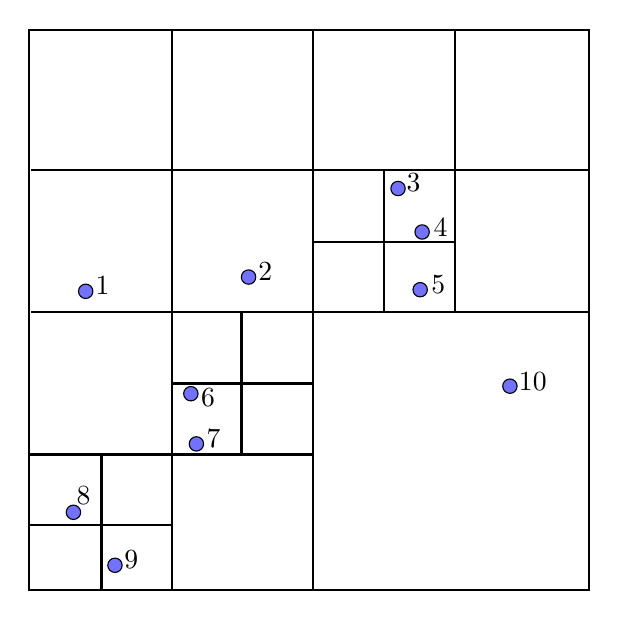
\begin{tikzpicture}[y=0.80pt, x=0.8pt,yscale=-0.5, xscale=0.5, inner sep=0pt, outer sep=0pt]
  \path[draw=black,line join=miter,line cap=butt,line width=0.800pt]
  (356.4286,94.5050) -- (356.4286,598.7908);
  \path[draw=black,line join=miter,line cap=butt,line width=0.800pt]
  (102.1429,348.7908) -- (605.7143,348.7908);
  \path[draw=black,line join=miter,line cap=butt,line width=0.800pt]
  (102.1429,220.2193) -- (607.1429,220.2193);
  \path[draw=black,line join=miter,line cap=butt,line width=0.800pt]
  (229.2857,93.0765) -- (229.2857,598.7908);
  \path[draw=black,line join=miter,line cap=butt,line width=0.800pt]
  (485.0000,93.7908) -- (485.0000,349.5050);
  \path[draw=black,line join=miter,line cap=butt,line width=0.800pt]
  (101.4286,477.3622) -- (356.4286,477.3622);
  \path[draw=black,line join=miter,line cap=butt,line width=0.800pt]
  (420.7143,220.2193) -- (420.7143,349.5050);
  \path[draw=black,line join=miter,line cap=butt,line width=0.800pt]
  (356.4286,285.2193) -- (485.0000,285.2193);
  \path[draw=black,line join=miter,line cap=butt,line width=0.800pt]
  (292.1429,348.0765) -- (292.1429,476.6479);
  \path[draw=black,line join=miter,line cap=butt,line width=0.800pt]
  (228.5714,413.0765) -- (357.1429,413.0765);
  \path[draw=black,line join=miter,line cap=butt,line width=0.800pt]
  (165.7143,477.3622) -- (165.7143,599.5050);
  \path[draw=black,line join=miter,line cap=butt,line width=0.800pt]
  (100.7143,540.9336) -- (229.2857,540.9336);
  \path[cm={{0.86607143,0.0,0.0,0.86607143,(-133.53636,-75.700851)}},draw=black,fill=c7372ff]
  (506.4286,453.4336)arc(0.000:180.000:7.500)arc(-180.000:0.000:7.500) -- cycle;
  \path[cm={{0.86607143,0.0,0.0,0.86607143,(-280.6792,-62.843726)}},draw=black,fill=c7372ff]
  (506.4286,453.4336)arc(0.000:180.000:7.500)arc(-180.000:0.000:7.500) -- cycle;
  \path[cm={{0.86607143,0.0,0.0,0.86607143,(-185.6792,29.656274)}},draw=black,fill=c7372ff]
  (506.4286,453.4336)arc(0.000:180.000:7.500)arc(-180.000:0.000:7.500) -- cycle;
  \path[cm={{0.86607143,0.0,0.0,0.86607143,(-180.6792,75.013418)}},draw=black,fill=c7372ff]
  (506.4286,453.4336)arc(0.000:180.000:7.500)arc(-180.000:0.000:7.500) -- cycle;
  \path[cm={{0.86607143,0.0,0.0,0.86607143,(-291.75062,136.79913)}},draw=black,fill=c7372ff]
  (506.4286,453.4336)arc(0.000:180.000:7.500)arc(-180.000:0.000:7.500) -- cycle;
  \path[cm={{0.86607143,0.0,0.0,0.86607143,(-254.25063,184.65628)}},draw=black,fill=c7372ff]
  (506.4286,453.4336)arc(0.000:180.000:7.500)arc(-180.000:0.000:7.500) -- cycle;
  \path[cm={{0.86607143,0.0,0.0,0.86607143,(102.53509,22.87056)}},draw=black,fill=c7372ff]
  (506.4286,453.4336)arc(0.000:180.000:7.500)arc(-180.000:0.000:7.500) -- cycle;
  \path[cm={{0.86607143,0.0,0.0,0.86607143,(21.463659,-64.272297)}},draw=black,fill=c7372ff]
  (506.4286,453.4336)arc(0.000:180.000:7.500)arc(-180.000:0.000:7.500) -- cycle;
  \path[cm={{0.86607143,0.0,0.0,0.86607143,(23.249374,-116.41515)}},draw=black,fill=c7372ff]
  (506.4286,453.4336)arc(0.000:180.000:7.500)arc(-180.000:0.000:7.500) -- cycle;
  \path[cm={{0.86607143,0.0,0.0,0.86607143,(1.4636592,-155.70087)}},draw=black,fill=c7372ff]
  (506.4286,453.4336)arc(0.000:180.000:7.500)arc(-180.000:0.000:7.500) -- cycle;
  \path[fill=black] (160.31509,332.78058) node[above right] (text6462) {1};
  \path[fill=black] (307.43341,319.70856) node[above right] (text6462-4) {2};
  \path[fill=black] (441.40405,239.94313) node[above right] (text6462-9) {3};
  \path[fill=black] (465.61832,280.30029) node[above right] (text6462-98) {4};
  \path[fill=black] (463.73944,332.14725) node[above right] (text6462-5) {5};
  \path[fill=black] (255.68974,433.98373) node[above right] (text6462-0) {6};
  \path[fill=black] (260.68976,470.65741) node[above right] (text6462-7) {7};
  \path[fill=black] (143.21951,522.34161) node[above right] (text6462-3) {8};
  \path[fill=black] (186.40405,580.65741) node[above right] (text6462-43) {9};
  \path[fill=black] (542.83264,419.586) node[above right] (text6462-02) {10};
  \path[draw=black,line join=miter,line cap=butt,line width=0.800pt]
  (606.0915,92.7173) -- (606.0915,599.8138) -- (100.0051,599.8138) --
  (100.0051,92.7173);
  \path[draw=black,line join=miter,line cap=butt,line width=0.800pt]
  (100.0051,93.7274) -- (605.0814,93.7274);
\end{tikzpicture}

  }
  \hspace{10pt}
  \subfloat[Tree representation]{
    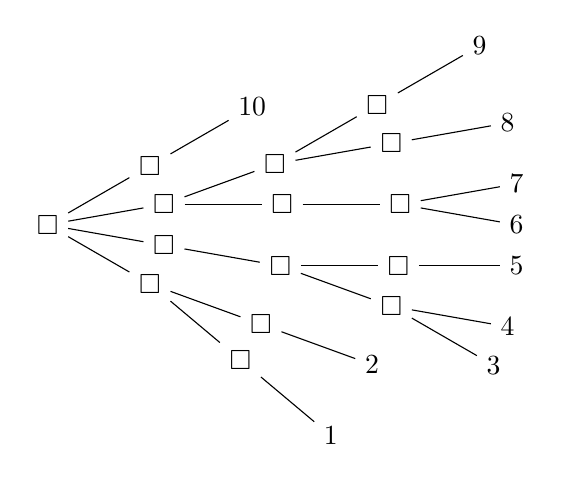
\begin{tikzpicture}[grow cyclic]
  \node {\square}
  child {
    node {\square}
    child {
      node {\square}
      child {node {1}}
    }
    child {
      node {\square}
      child {node {2}}
    }
  }
  child {
    node {\square}
    child {
      node {\square}
      child {
        node {\square}
        child { node{3} }
        child { node{4} }
      }
      child {
        node {\square}
        child {node{5}}
      }
    }
  }
  child {
    node {\square}
    child {
      node {\square}
      child {
        node {\square}
        child {node{6}}
        child {node{7}}
      }
    }
    child {
      node {\square}
      child {
        node {\square}
        child {node{8}}
      }
      child {
        node {\square}
        child {node{9}}
      }
    }
  }
  child {
    node {\square}
    child { node {10} }
  }
  ;
\end{tikzpicture}

  }
  \caption{The QuadTree for a sample graph, empty branches omitted}
  \label{fig:quadtree}
\end{figure}

The first step is to build a data structure representing the recursive
subdivision. This kind of data structure is called a \code{TreeCode},
which recursively subdivides the space until only one node remains in
the current space, or a maximum depth/minimum space size size is
hit. The space decomposition can be irregular (e.g. \emph{Voronoi}
spaces) or regular. In the latter case, the space is recursively
subdivided in squares. We chose to use a regular, 4-way space
decomposition, mainly due to its simplicity. This kind of structure is
called \code{QuadTree}. Figure \ref{fig:quadtree} shows a sample
QuadTree for a Visigoth graph. In the QuadTree, each sub-quadrant
preserved the weighted centre of gravity relative to the contained
nodes.

Building the tree is the difficult part of the algorithm and can be
done in linear time.  Once that is done, to calculate the non-edge
forces for a given node the algorithm proceeds as indicated in figure
\ref{proc:FADE}.

\begin{figure}[ht]
  \begin{minipage}[b]{0.5\linewidth}
    \begin{algorithmic}
  \REQUIRE \(0 < \theta < 1\)
  \REQUIRE \(\beta > 1\)
  \REQUIRE \(\vec{n} \neq \vec{q}\)
\end{algorithmic}
force\((n, q)\):
\begin{algorithmic}
  \STATE \(\vec{d} \gets \vec{n} - \vec{q}\)
  \IF { \(q\) is terminal \OR \(\frac{\vec{d}}{\textrm{width}(q)} < \theta\) }
  \STATE \(\vec{v} \gets \vec{d} \cdot \frac{\beta}{|{\vec{d}}|^2}\)
  \STATE \(\vec{v} \gets \vec{v} \cdot \textrm{mass}(q)\)
  \RETURN \(\vec{v} \cdot \frac{\beta}{|{\vec{d}}|^2}\)
  \ELSE
  \STATE \(\vec{v} \gets 0\)
  \FOR {\(q'\) in children\((q)\)}
  \STATE \(\vec{v} \gets \vec{v} + \textrm{force}(n, q')\)
  \ENDFOR
  \RETURN \(\vec{v}\)
  \ENDIF
\end{algorithmic}

    \caption{This procedure calculates the non-edge force of a given
      node \(n\), given the QuadTree \(q\). \(\vec{n}\) and
      \(\vec{q}\) indicate the vectors corresponding to the respective
      centers of gravity. \(\beta\) is an empirically determined
      parameter used to regulate the amount of force - \(75\) has
      worked well for us. \(\theta\) is central to the \FADE algorithm
      and determines the amount of approximation. If \(\geq 1\) the
      algorithm is unstable, we used values between \(0.5\) and
      \(0.8\). See figure \ref{fig:theta} for a visual
      explanation. The mass of a quadrant is simply the number of
      nodes residing in it. }
    \label{proc:FADE}
  \end{minipage}
  \hspace{10pt}
  \begin{minipage}[b]{0.5\linewidth}
    \centering
    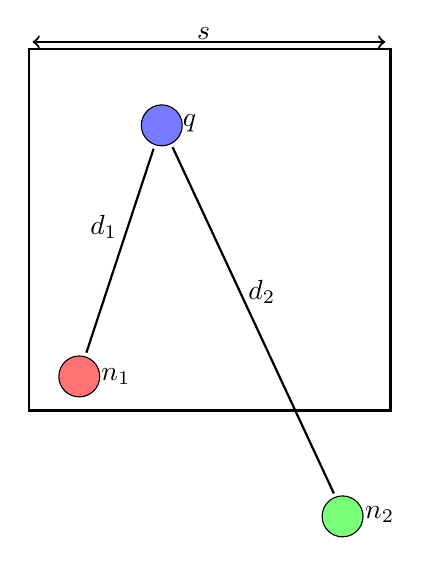
\begin{tikzpicture}[y=0.80pt, x=0.8pt,yscale=-1, inner sep=0pt, outer sep=0pt]
  \path[draw=black,fill=cffffff,line join=miter,line cap=butt,fill
    opacity=0.000,even odd rule,line width=0.803pt,rounded corners=0.0000cm]
  (140.4134,176.5621) rectangle (303.7579,339.9066);
  \path[cm={{0.79503474,0.0,0.0,0.79503474,(-296.23722,-12.403676)}},draw=black,fill=c787aff]
  (636.3961,281.1107)arc(0.000:180.000:11.617)arc(-180.000:0.000:11.617) --
  cycle;
  \path[cm={{0.79503474,0.0,0.0,0.79503474,(-333.50701,101.01225)}},draw=black,fill=cff7374]
  (636.3961,281.1107)arc(0.000:180.000:11.617)arc(-180.000:0.000:11.617) --
  cycle;
  \path[cm={{0.79503474,0.0,0.0,0.79503474,(-214.57843,164.22654)}},draw=black,fill=c79ff79]
  (636.3961,281.1107)arc(0.000:180.000:11.617)arc(-180.000:0.000:11.617) --
  cycle;
  \path[draw=black,line join=miter,line cap=butt,line width=0.800pt]
  (166.4286,313.7908) -- (196.7857,221.6479);
  \path[draw=black,line join=miter,line cap=butt,line width=0.800pt]
  (205.3571,220.9336) -- (278.2143,377.3622);
  \path[fill=black] (168.21428,262.36218) node[above right] (text5235) {\(d_1\)};
  \path[fill=black] (239.64287,291.64789) node[above right] (text5239) {\(d_2\)};
  \path[fill=black] (216.42857,172.36218) node[above right] (text5243) {\(s\)};
  \path (142.5000,173.7908) -- (300.0000,173.7908);
  \path[draw=black,line join=miter,line cap=butt,line width=0.800pt, <->]
  (142.1429,173.4336) -- (301.4286,173.4336);
  \path[fill=black] (210,214.1479) node[above right] (text5479) {\(q\)};
  \path[fill=black] (173.21429,328.07648) node[above right] (text5483) {\(n_1\)};
  \path[fill=black] (292.34625,390.3728) node[above right] (text5483-5) {\(n_2\)};
\end{tikzpicture}

    \caption{In this case, \(n_1\) and \(n_2\) are nodes and \(q\) is
      a quadrant with edge length \(s\). When calculating the non-edge
      force between \(n_1\) and \(q\), where \(s\) is the quadrant
      will be judged to be too close to approximate, since
      \(\frac{s}{d_1} > 1\), while \(n_2\) might be judged far enough,
      depending on \(\theta\).}
    \label{fig:theta}
  \end{minipage}
\end{figure}

Once implemented, the \FADE algorithm lead to great speedups while
preserving good node placements. While drawing \(1000\) nodes is
already difficult with the simple algorithm, \FADE can easily handle
\(10000\) nodes, after which other performance limits are hit (the
graph generation time and the OpenGL drawing).

However, once we implemented the 3D view we had to temporarily switch
back to the naive algorithm, since the 3D positioning requires heavy
modifications to \FADE, which we planned to do in the near future.

\section{Looking back}
%% This section corresponds to D in the requirements

\subsection{Validation}
%% The client is a happy puppy

\subsection{Lessons learned}

\addcontentsline{toc}{section}{References}
\begin{thebibliography}{9}

\bibitem{hamm10}
  David A. Hammond,
  \emph{Altruism in Small World Models}.
  Imperial College London,
  2010.

\bibitem{oconn11}
  Luke M. O'Connor,
  \emph{Algorithms for Constructing Realistic Networks}.
  Imperial College London,
  2011.

\bibitem{fade}
  Aaron Quigley and Peter Eades,
  \emph{FADE: Graph drawing, clustering and visual abstraction}.
  Department of Computer Science and Software Engineering,
  Univ. of  Newcastle, Australia, 2000.

\end{thebibliography}

\end{document}
